\section{Definition}
\label{definition:definition}
\subsection{Message Oriented Middleware}
Eine \textit{Message Oriented Middleware} (kurz MOM), also eine
nachrichtenorientierte Middleware, wird definiert als eine beliebige Middleware,
die es ihren \textit{Clients} ermöglicht, Nachrichten aneinander zu versenden \cite{tanenbaum2007distributed}.
Diese entkoppelt Sender und Empfänger (in diesem Kontext auch
\textit{Producer} und \textit{Consumer} genannt \cite{eugster2003many}), da nun nicht
mehr alle Teilnehmer untereinander verbunden sein müssen, sondern nur noch mit
der Middleware.
Dies wird in den Darstellungen \ref{Message Broker:rpcvsmom} abgebildet.
Hierbei wird in beiden Fällen die Netzwerkarchitektur gezeigt, die benötigt wird,
damit jeder Teilnehmer an jeden anderen Teilnehmer Nachrichten senden kann.
Dargestellt sind Clients bzw. bei (b) Clients und in der Mitte eine MOM.

Dabei beschreibt der Begriff Message Oriented Middleware keine konkrete Umsetzung.
Eine solche besteht in den meisten modernen Implementierungen aus einem oder
mehreren Brokern, die nach einem gewissen Schema routen sowie Queues, die
Nachrichten speichern können. Diese Strukturen werden in den nächsten Abschnitten
detailliert erklärt. \cite{curry2004message}

\begin{figure}[h]
  \centering
  \begin{subfigure}{.49\textwidth}
    \centering
    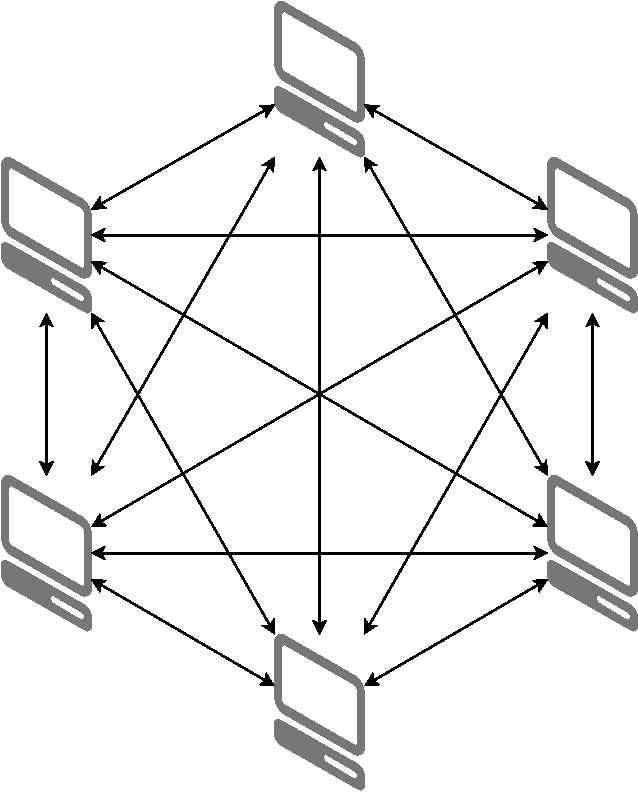
\includegraphics[width=0.5\textwidth]{figures/rpc.pdf}
    \caption{Aufbau ohne MOM}
    \label{Message Broker:rpcvsmom:rpc}
  \end{subfigure}
  \begin{subfigure}{.49\textwidth}
    \centering
    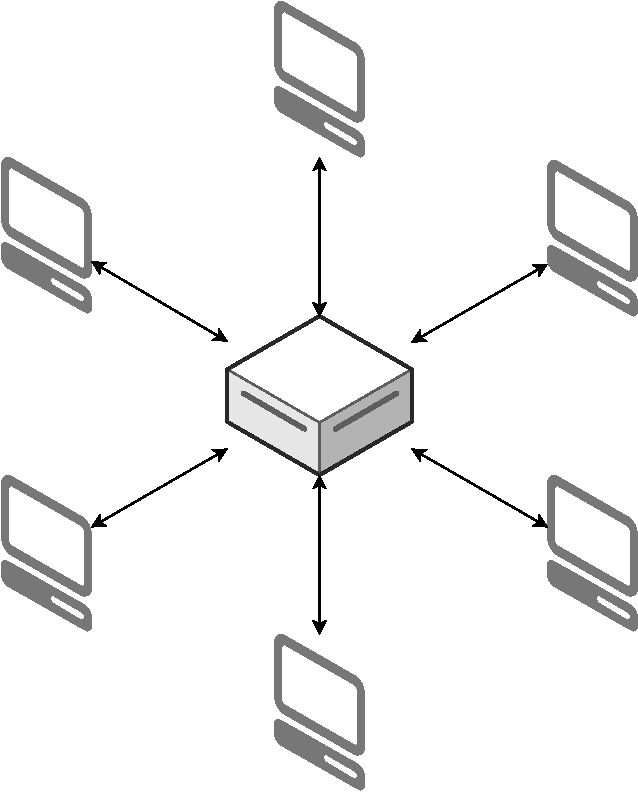
\includegraphics[width=0.5\textwidth]{figures/broker.pdf}
    \caption{Aufbau mit MOM}
    \label{Message Broker:rpcvsmom:mom}
  \end{subfigure}
  \caption{Netzwerkarchitektur bei Verwendung direkter Kommunikation im Vergleich mit einer Message Oriented Middleware}
  \label{Message Broker:rpcvsmom}
\end{figure}

Ein \textit{Message Broker} sorgt für das Weiterleiten der Nachrichten an den
richtigen Empfänger. Dabei kann er auch Nachrichten, die in
einem bestimmten Format angenommen wurden, in ein anderes, zum Empfänger
kompatibles Format umwandeln. Er sorgt also für eine Entkopplung von
Nachrichtenformaten.
Bei der Verwendung eines Brokers werden alle Nachrichten über diesen geleitet. 
Er verarbeitet die Nach\-richten und leitet sie nach gewissen Regeln weiter.
Man spricht auch von einem \textit{Routing}, hierauf wird in Abschnitt 
\ref{definition:routing} näher eingegangen. \cite{tanenbaum2007distributed}

Eine Queue ist im Kontext von MOM eine Speicherlösung für Nachrichten.
Dabei können je nach Implementierung eine oder mehrere Queues für die gesamte
MOM existieren. Auch ob eine Queue vor den
Message Broker geschaltet wird, oder dieser seine Nachrichten an eine Queue
weiterleitet, ist implementierungsabhängig \cite{KafkaClients:online,RabbitMQ:online}.
Warum Queues verwendet werden und welche Vorteile dies haben kann, wird in
Abschnitt \ref{definition:queues} besprochen.
Eine Veranschaulichung eines exemplarischen Gesamtaufbaus einer MOM mit den
eben besprochenen Teilen ist in Darstellung \ref{definition:momfigure} zu finden.
Hierbei ordnet der Message Broker die empfangenen Nachrichten in eine der Queues
ein, von denen die Consumer diese erhalten.

\begin{figure}[h]
  \centering
    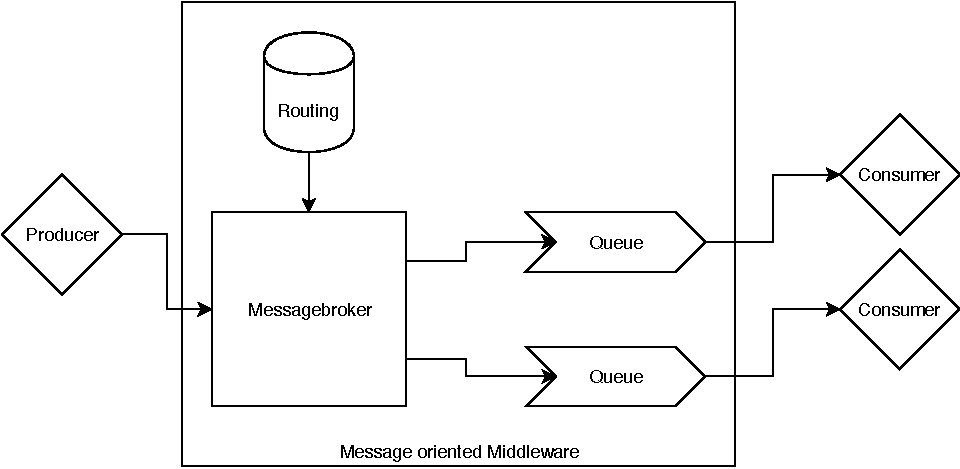
\includegraphics[width=0.9\textwidth]{figures/mom.pdf}
  \caption{Exemplarischer Aufbau einer Message Oriented Middleware}
  \label{definition:momfigure}
\end{figure}

Ein großer Vorteil, den eine MOM bieten kann, ist \textit{asynchrone} Kommunikation.
Ist eine Architektur synchron, so wird bei dem Verschicken der
Nachricht der weitere Ablauf des Senders blockiert, bis eine Antwort erhalten
und der Ablauf fortgesetzt wird. Bei der asynchronen Variante kann eine
Nachricht verschickt werden, ohne dass der Ablauf dadurch blockiert wird.
Dies ist vor allem in Batchverarbeitungs- und parallelen Systemen nützlich \cite{tanenbaum2007distributed}.
Zur Veranschaulichung dient Abbildung \ref{Message Broker:communication}, in
der der asynchrone Versand einer Nachricht dargestellt ist. Dabei wird die erste
Nachricht von \textit{Client 2} verarbeitet und danach eine Antwort verschickt.
Weitere Vorteile werden in Abschnitt \ref{Message Broker:advantages} besprochen.

In den untersuchten Implementierungen findet dabei das \textit{Publish-Subscribe}
Pattern Anwendung. Es beschreibt die Art, wie sich zwei verschiedene Teile einer
Software miteinander verbinden und kommunizieren. Dabei ist bei Publish-Subscribe
(kurz auch PubSub) eine Nachricht nicht an einen Empfänger direkt gerichtet,
sondern Sender können Nachrichten veröffentlichen (publish) und interessierte
Empfänger können ihr Interesse durch eine Subscription bekunden.
Daraufhin erhalten alle Subscriber, beispielsweise eines bestimmten Themas, alle
Nachrichten davon. Auf welche Art diese Auswahl stattfindet, wird genauer im nächsten
Abschnitt (\ref{definition:routing} Routing) beschrieben. \cite{eugster2003many}

\begin{figure}[h]
  \centering
    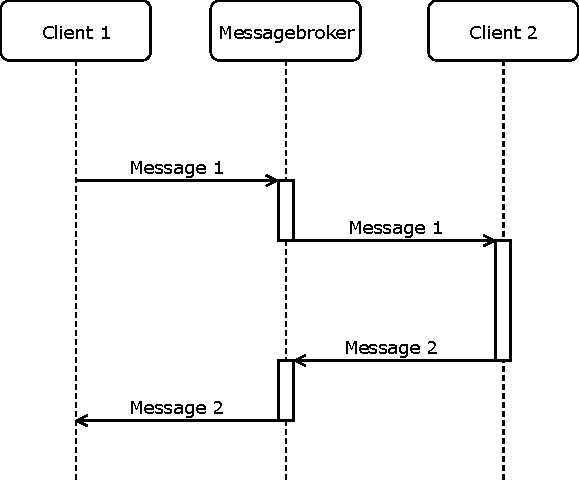
\includegraphics[width=0.5\textwidth]{figures/communication.pdf}
  \caption{Asynchrone Kommunikation mithilfe eines Message Brokers}
  \label{Message Broker:communication}
\end{figure}

\subsection{Routing}
\label{definition:routing}
Message Broker müssen architekturbedingt ein Regelwerk anbieten, nach dem Nachrichten
bestimmten Empfängern zugestellt werden, da die Nachrichten nicht direkt an diese
geschickt werden. Man spricht von einem \textit{Routing}.
So kann man neben statisch festgelegten Routen auch \textit{Channel-},
\textit{Topic-}, oder \textit{Content-}basiert geroutet werden \cite{tanenbaum2007distributed}.
Bei channelbasiertem Routing werden Kanäle gebildet, denen Clients beitreten können;
daraufhin erhalten diese alle in dem Kanal veröffentlichten Nachrichten.
Eine weitere Möglichkeit ist das Bilden von \textit{Topics}, wodurch dann je
nach thematischer \textit{Subscription} des einzelnen Clients Nachrichten zugestellt werden
\cite{eugster2003many}.
Bei inhaltsbasiertem Routing wird basierend auf dem Inhalt der einzelnen Messages vom
Broker beurteilt, welche Consumer diese erhalten \cite{tanenbaum2007distributed}.

Dabei sind je nach Protokoll und Implementierung verschiedene Ausprägungen anzutreffen.
Die meisten bieten mindestens eine Topic-Logik, oft auch eine Bildung von Channels an.
Sie unterscheiden sich hauptsächlich darin, wie mit mehreren Topics umgegangen wird.
Es können beispielsweise Wildcards verwendet oder logische Verknüpfungen
erstellt werden.
Wenn z.B. gewünscht ist, dass ein Consumer alle Topics der Nachricht 
abonniert haben muss, um diese zu erhalten, kann dies unter anderem mit
RabbitMQ bzw. dem verwendeten AMQP-Protokoll realisiert werden \cite{dobbelaere2017kafka}.
Weitere Details zu den jeweiligen Routingoptionen werden im Abschnitt
\ref{part:comparison} für die einzelnen Implementierungen besprochen.

\subsection{Queues}
\label{definition:queues}
Um eine stärkere Entkopplung zu erreichen, werden in modernen Implementierungen
häufig Queues verwendet.
Im Kontext von Message Oriented Middleware sind hier mit Queues
Speicher für Nachrichten gemeint \cite{curry2004message}.
Je nach Implementierung wird eine Nachricht hier nur zwischengespeichert, bis
sie erfolgreich weitergeleitet wurde, oder dauerhaft gespeichert.
Dies hat zwei Vorteile. Zum einen können bei einer langsamen Abarbeitung von
den Consumern die Nachrichten zwischengespeichert werden, und gehen nicht verloren.
Zum anderen kann eine langfristige Speicherung beispielsweise als Backup fungieren.
Dabei stößt man auf die üblichen Prinzipien von Warteschlangen. Im Kontext von
nachrichtenorientierten Middlewares ist eine Queue meistens ein \textit{FIFO},
gibt also die Nachrichten nach dem Zwischenspeichern in unveränderter Reihenfolge
wieder an den Empfänger aus \cite{curry2004message}.
Es existieren jedoch Lösungen wie Kafka, bei denen zwar eine Ordnung innerhalb
einzelner Queues vorliegt, jedoch die Broker zusätzlich zu ihrer normalen
Publish-Subscribe Kommunikation auch gezielt beliebige gespeicherte Nachrichten
abrufen können. Hierbei kann also nicht nach üblichen Kriterien von
Warteschlangen bewertet werden \cite{ApacheKa84:online}.
Wie bereits erwähnt, ist es abhängig von der Implementierung, wie die Queue
mit dem Rest der MOM zusammenarbeitet. Details hierzu werden im Abschnitt
\ref{part:comparison} für die jeweilige Implementierung besprochen.

\subsection{Protokolle}
Je nach Implementierung werden verschiedene Protokolle verwendet und unterstützt.
Dabei existieren komplett proprietäre Protokolle bzw. Eigenentwicklungen, wie zum
Beispiel bei ZeroMQ oder Kafka \cite{ApacheKa84:online}. 
Abseits hiervon hat sich vorerst vor allem \textit{JMS}, das Java Message
Service Protokoll, durchgesetzt. Dies wird in ActiveMQ, JBOSS Messaging und
einigen anderen Implementierungen verwendet \cite{dobbelaere2017kafka}.
Als populäres und standardisiertes Protokoll ist auch \textit{AMQP},
Advanced Message Queueing Protocol, hervorzuheben \cite{vinoski2006advanced}.
Es findet in RabbitMQ, Qpid, HornetMQ und Weiteren Verwendung \cite{dobbelaere2017kafka}.
Daneben gibt es noch weitere Protokolle wie NMS, STOMP und WebSocket, allerdings
wird in der Industrie hauptsächlich AMQP verwendet. \cite{vinoski2006advanced}
Erwähnenswert ist jedoch noch MQTT (Message Queue Telemetry Transport), ein
im IoT-Bereich weit verbreitetes Protokoll. Es zeichnet sich durch seine
Leichtgewichtigkeit und einfache Implementierung aus \cite{dobbelaere2017kafka}.

AMQP ist ein offener Standard, um Nachrichten zwischen zwei Anwendungen
auszutauschen. 
Es wurde durch eine Arbeitsgruppe zusammengestellt und Anfang 2010 in seiner
ersten Version präsentiert.
Um von der großen Verbreitung von JMS profitieren zu können, wurde für Kompatibilität
gesorgt \cite{vinoski2006advanced}. Somit kann AMQP auch in einer JMS-Umgebung
integriert werden, um von AMQPs erhöhter Kompatibilität mit weiterer Software
profitieren zu können.
AMQP legt fest, wie die Kommunikation zwischen den Clients und den Brokern abläuft,
jedoch nicht, was der Broker tut. Daher können verschiedene Broker untereinander
unterschiedliche Funktionalitäten zur Verfügung stellen und trotzdem AMQP
unterstützen.

Die meisten Protokolle sind Netzwerkprotokolle und arbeiten auf der Anwendungsebene.
Sie umfassen dabei Spezifizierungen darüber, wie die Nachrichten verschickt werden.
Im Falle von AMQP wurde dies mit einem binären Peer-to-Peer Protokoll umgesetzt.
Weiter wird meistens ein bestimmtes Nachrichtenformat vorgegeben, nach denen alle
in der MOM propagierten Nachrichten strukturiert sind. Hierbei liegen auch die
Unterschiede in Protokollen, da sie erstens noch weitere Teile des
Kommunikationsprozesses standardisieren, und zweitens unterschiedliche
Spezifizierungen für Übertragung und Nachrichtenformat mitbringen können.
\cite{vinoski2006advanced}
